\documentclass[dvipdfmx]{jarticle}
\pagestyle{empty}
\usepackage{tikz}
\usetikzlibrary{calc,shapes,arrows.meta}
\usepackage{fancyvrb}
\usepackage{array}
\begin{document}
    \begin{tabular}{ccc}
        \begin{minipage}{.3\linewidth}
            \begin{Verbatim}
                t=1
                n=10
                L1: t=t*n
                n=n-1
                b=(n>1)
                if b goto L1
                f=t
            \end{Verbatim}
        \end{minipage}
         & \hspace*{3cm} &
        \begin{minipage}{.4\linewidth}
            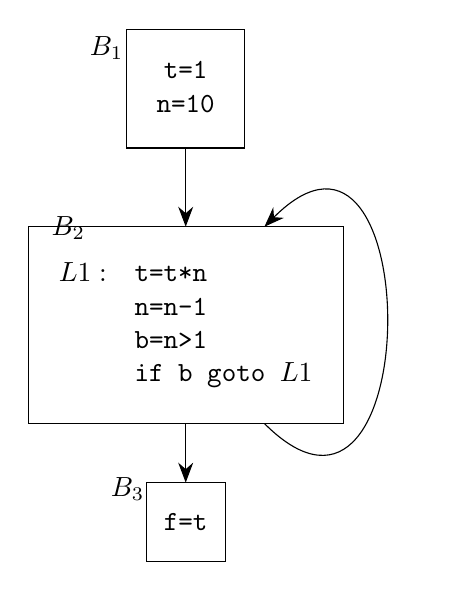
\begin{tikzpicture}
                \node[label={160:{$B_1$}}] (B1) at (0,0) {$\begin{array}{c}
                                \texttt{t=1} \\
                                \texttt{n=10}
                            \end{array}$};
                \draw ($(B1)+(-0.75,0.75)$) rectangle +(1.5,-1.5);
                \node[label={140:{$B_2$}}] (B2) at ($(B1)+(0,-3)$) {$\begin{array}{ll}
                                L1: & {\texttt{t=t*n}}           \\
                                    & {\texttt{n=n-1}}           \\
                                    & {\texttt{b=n>1}}           \\
                                    & {\texttt{if\ b\ goto\ }L1}\end{array}$};
                \draw ($(B2)+(-2,1.25)$) rectangle +(4,-2.5);
                \node[label={160:{$B_3$}}] (B3) at ($(B2)+(0,-2.5)$) {$\texttt{f=t}$};
                \draw ($(B3)+(-0.5,0.5)$) rectangle +(1,-1);
                \draw[-{Stealth[scale=1.5]}] ($(B1)+(0,-0.75)$) -- ($(B2)+(0,1.25)$);
                \draw[-{Stealth[scale=1.5]}] ($(B2)+(0,-1.25)$) -- ($(B3)+(0,0.5)$);
                \path[-{Stealth[scale=1.5]},out=315,in=45,looseness=3.0] ($(B2)+(1,-1.25)$) edge ($(B2)+(1,1.25)$);
            \end{tikzpicture}
        \end{minipage}
    \end{tabular}
\end{document}